\documentclass[12pt,a4paper]{article}
\usepackage[utf8]{inputenc}
\usepackage[brazil]{babel}
\usepackage{geometry}
\usepackage{amsmath}
\usepackage{amssymb}
\usepackage{graphicx}
\usepackage{enumitem}
\usepackage{titlesec}
\usepackage{fancyhdr}
\usepackage{indentfirst}

% Configurações de página
\geometry{a4paper, left=2.5cm, right=2.5cm, top=2.5cm, bottom=2.5cm}

% Formatação de seções
\titleformat{\section}{\large\bfseries}{\thesection}{1em}{}
\titleformat{\subsection}{\normalsize\bfseries}{\thesubsection}{1em}{}

% Configuração do cabeçalho
\pagestyle{fancy}
\fancyhf{}
\fancyhead[L]{\textbf{AGG0327}}
\fancyhead[R]{\textbf{Atividade 1}}
\fancyfoot[C]{\thepage}

\begin{document}
\thispagestyle{fancy}

\begin{center}
    \textbf{AGG0327 – Sismica de Reflexão \hfill Atividade 1 \hfill Entrega até 28/10/25}
\end{center}

\vspace{0.3cm} % Espaço reduzido

\textbf{Nome:} Gabriel Aparecido das Chagas Silva 14571098

\vspace{0.3cm} % Espaço reduzido

\begin{center}
    \textbf{Prática Computacional: Edição da geometria de aquisição CMP}
\end{center}


\section{Geometria de aquisição convencional da técnica CMP.}

Considere as seguintes informações sobre os parâmetros de aquisição CMP:
\begin{itemize}[leftmargin=2cm]
    \item \textbf{Aquisição CMP convencional:} movimentação dos tiros e dos geofones, \textbf{mantendo o afastamento mínimo constante}
    \item \textbf{Afastamento mínimo:} 10 m
    \item \textbf{Intervalo de geofones:} 10 m
    \item \textbf{Intervalo entre pontos de tiro:} 20 m
    \item \textbf{Coordenada do primeiro tiro:} 0 m
    \item \textbf{Multiplicidade do levantamento:} 24
\end{itemize}

\subsection{I.1) Questões:}


Seja $M$ a multiplicidade, $N$ o número de geofones, $dx$ o espaçamento dos geofones e $d$ a distância entre os tiros, temos que a multiplicidade se dá por:

\begin{equation}
    M = \frac{N\cdot dx}{2d}
\end{equation}


A partir de (1) pode-se obter o número de geofones utilizados esse levantamento: $$N = \frac{2Md}{dx} \implies N =\frac{ 2\cdot 24 \cdot 20}{10} = 96$$




\subsubsection{1) Qual a coordenada (em metros) do CMP 1 (cdp=1)?}

Sendo o primeiro tiro $X_s = 0m$ e $X_g = 10m$ a posição do primeiro geofone de acordo com o offset mínimo, temos que a posição do primeiro CDP (CMP 1) é $$X_{CDP} = \frac{X_s + X_g}{2} = 5m$$.




\subsubsection{2) Qual o número do CMP do primeiro traço do tiro 2?}

Um tiro, em um arranjo com 96 geofones, vai ter 96 traços em cada um deles. Sendo o intervalo entre os tiros $\Delta d = 20m$, o tiro 2 se encontra na posição $X_S = 20m$, enquanto o primeiro geofone (responsável pelo primeiro traço) se encontra na posição, em relação ao tiro, de $$X_g = 20m + 10m = 30m$$. Logo, obtém-se o valor de posição do CMP de $$X_{CMP} = \frac{30+20}{2} = 25m$$. Levando em consideração que o intervalo entre os CDP's é dado por 

\begin{equation}
    \Delta CMP =  CMP_{i+1} -  CMP_{i} = \frac{\Delta X_g}{2}
\end{equation}

\noindent

,obtém-se o intervalo entre os CMP's de $5m$. Como a posição do CMP do primeiro traço no tiro 2 é de $25m$, o número do CMP é $5$, já que $5 \cdot 5 = 25$.


\subsubsection{3) Qual o número e a coordenada do primeiro CMP com 3 traços?}


O primeiro CMP com 3 traços é o primeiro CMP que teve 3 pares fonte-geofone que possuem o mesmo ponto médio. A posição do CMP do tiro 2 está em $25m$ e corresponde ao CMP 5; o primeiro CMP com três traços será o primeiro ponto amostrado pelo tiro 3. Como o número do CMP do primeiro geofone do primeiro tiro é 1 e o CMP do primeiro geofone do segundo tiro é 5, pela camada ser plana, pode-se considerar o intervalo entre os CMP's para cada geofone de $5-1 = 4$ geofones, também obtido pela relação 

\begin{equation}
    \frac{Tiro}{CDP} = \frac{\Delta d}{\Delta X_{CDP}}
\end{equation}

\noindent
que diz quantos CDP's são 'pulados' a cada tiro. Logo, para o tiro 3, calcula-se

$$ \frac{20}{5} = 4$$

Sabendo disso, o primeiro CMP com três traços será o do tiro 3, e somando 4 ao primeiro CMP do segundo tiro obtemos $5 + 4 = 9$. Generalizando a equação para determinar qualquer CDP com n traços:

\begin{equation}
    CDP_n = CDP_1 + (n-1) \cdot Pulo
\end{equation}

\noindent
sendo $Pulo$ a equação (3). Para saber a coordenada correspondente, pode-se converter (4), que retorna um índice, em coordenadas em metros, por meio da multiplicação do valor do pulo pelo intervalo entre cada índice do CDP (no caso dessa questão, 5m):

\begin{equation}
    X_n = X_1 + (n-1) \cdot(Pulo \cdot \Delta CMP)
\end{equation}

A partir da equação acima, obtemos $X_3 = 45m$, no $CDP = 9$.



\subsubsection{4) Qual o número do primeiro CMP com 24 traços?}

A partir de (4), calcula-se

$$ CDP_{24} = 1 + (24-1) \cdot 4 = 93$$

O número do primeiro CMP é $93$. 


\subsubsection{5) Qual deve ser o número de geofones em cada ponto de tiro para que a multiplicidade máxima do levantamento seja 24 (2400\%)?}

A partir de (1), 96 geofones. 



\subsection{I.2) Geometria de aquisição no cabeçalho:}

O arquivo \texttt{null.su} contém o número de traços do levantamento. Não contém dados, todas as amostras possuem amplitude igual a zero; o arquivo foi gerado apenas para simular o volume de dados registrados no levantamento.

\subsubsection{1) Quais palavras-chave (keywords) existem nos cabeçalhos do arquivo?}

Nenhuma palavra-chave de geometria (como sx, gx, cdp) está definida ainda; os cabeçalhos estão zerados, o plot está ilustrado na figura 1.


\begin{figure}[h]
    \centering
    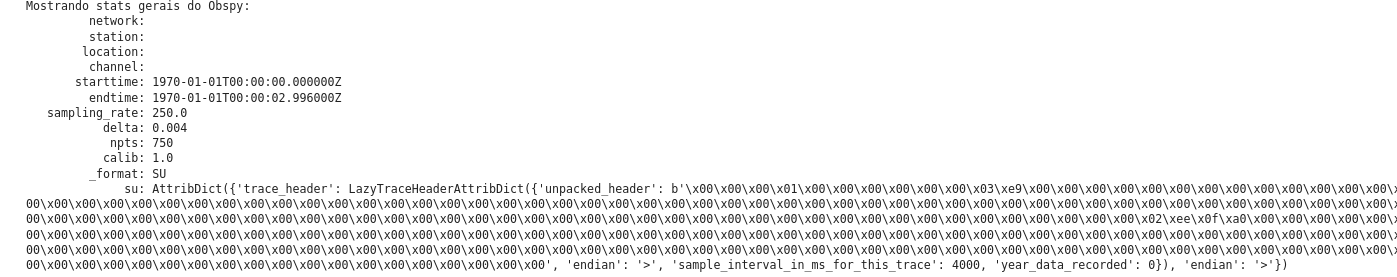
\includegraphics[width=0.5\linewidth]{cabecalho.png}
    \caption{Enter Caption}
    \label{fig:placeholder}
\end{figure}


\subsubsection{2) Insira nos cabeçalhos as palavras-chave: sx, gx, offset, ep, cdp.}
Para tal defina os seguintes parâmetros do programa \texttt{sushw}: (Escreva aqui os valores que utilizou)

\begin{itemize}[leftmargin=2cm]
    \item \texttt{key=sx,gx,offset,ep,cdp}
    \item \texttt{a=} 10 (offset mínimo)
    \item \texttt{b=} 10 (intervalo entre geofones)
    \item \texttt{c=} 20 (intervalo entre tiros)
    \item \texttt{j=} 96 (número de geofones) 
\end{itemize}

e execute o programa com a sintaxe abaixo (ou, substitua as variáveis com os valores diretamente na linha de comando a seguir):

\begin{quote}
\texttt{sushw <null.su key=\$key a=\$a b=\$b c=\$c j=\$j >null-geometria.su}
\end{quote}

\subsection{I.3) Visualize a carta de empilhamento para a geometria de aquisição acima.}

\begin{itemize}[leftmargin=2cm]
    \item \texttt{n=} 96 (é o número de geofones)
    \item \texttt{nplot=} 500 (é o número de pontos de tiro)
\end{itemize}

\begin{quote}
\texttt{suchart < null-geometria.su key1=ep key2=cdp | xgraph n=\$n nplot=\$nplot marksize=5 mark=0 linewidth=0 x1beg=0 x2beg=0 label1=ep label2=cdp \&}
\end{quote}

Escreva os valores utilizados para os números de geofones e de pontos de tiro.

Faça um printscreen da imagem da carta de empilhamento (anexe no Moodle o arquivo com a imagem da carta de empilhamento).


\begin{figure}[h]
    \centering
    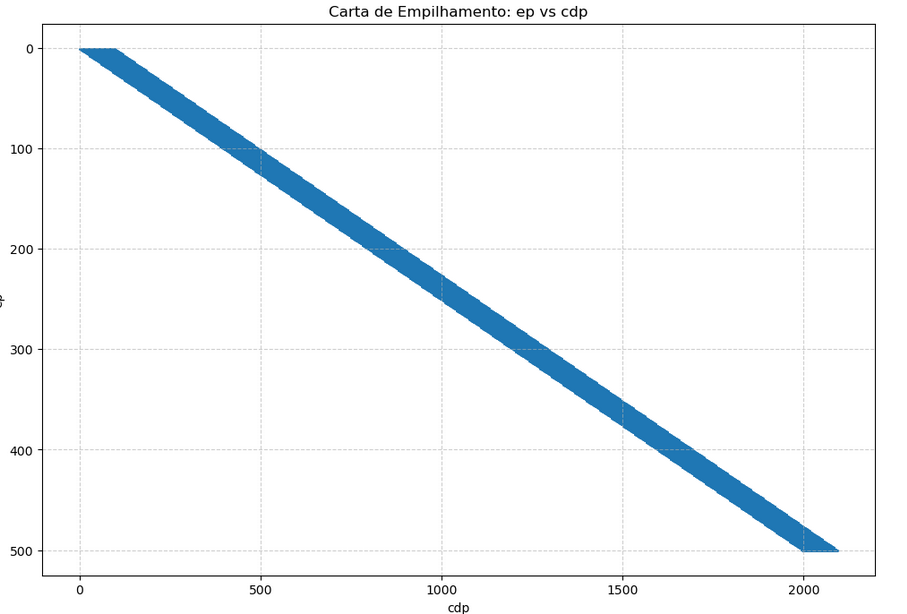
\includegraphics[width=0.75\linewidth]{carta.png}
    \caption{Carta de empilhamento}
    \label{fig:placeholder}
\end{figure}



\subsection{I.4) Questões:}

\subsubsection{1) Qual o intervalo (dx) entre os traços dentro de um sismograma CMP (dx = intervalo do offset)?}


Sabe-se que o offset $\rho$ é dado por 

\begin{equation}
    \rho = X_G - X_S
\end{equation}

Isolando $X_G$ obtemos $X_g = X_S + \rho$. Substituindo na equação da coordenada do CDP:

$$ X_{CDP} = \frac{X_S + X_G}{2} = X_S + \frac{\rho}{2}$$

Calculando as coordenadas do CDP para tiros A e B adjascentes:

\begin{itemize}
    \item Tiro A: $X_{CDP}  = X_{SA} + \frac{\rho_A}{2}$
    \item Tiro B: $X_{CDP}  = X_{SB} + \frac{\rho_B}{2}$
\end{itemize}


Igualando as equações dos tiros, sabendo que $X_{SB} = X_{SA} + \Delta X_S$ sendo $\Delta X_S$ o intervalo entre as fontes, obtém-se a relação:

$$ \rho_A = 40 + \rho_B \implies 40 = \rho_a - \rho_b$$

Logo, $40m$ é o intervalo entre os traços do sismograma. 





\subsubsection{2) Qual o comprimento da linha sísmica em superfície?}



A posição do primeiro tiro está em $0m$. Sabendo que o espaçamento entre os tiros é de $20m$, o último tiro estará na posição $20 \cdot 499 = 9680m$ levando em consideração os 500 pontos de tiro. O último dos 96 geofones estará na posição $96\cdot10 = 960m$ em relação ao começo do offset de 10 metros. Logo, o comprimento total da linha é de $9980 + 960 = 10940m$.




\subsubsection{3) Quais as coordenadas do início e final da amostragem em subsuperfície com máxima multiplicidade?}

A multiplicidade é de $24$. O primeiro CMP com 24 traços está no CMP $93$. é necessário achar o último CMP com essa multiplicidade. 

A coordenada do CMP $93$ é calculada com a equação (5) e resulta em $460m$, que é a largura da base do triângulo que se forma estabelecendo uma reta vertical nesse ponto, obtendo um triângulo retângulo. Podemos obter a coordenada do último CMP com base nos valores máximos da fonte e da posição dos geofones, estabelecendo como origem a extremidade esquerda no arranjo dos tiros, e o final a extremidade direita dos geofones. Utilizando os dados da questão anterior:

$$X_{CDP} = \frac{9980 + 10940}{2} = 10460m$$

Sendo essa a coordenada do último CMP. Subtraindo o valor da base do triângulo, chegamos à reta vertical do começo da multiplicidade máxima, a partir do referencial dos pontos com maiores CMD no gráfico de QC. Dessa forma, essa reta está localizada na posição $10460 - 460 = 10000m$. Portanto, a coordenada inicial é $460m$ e a final é $10000m$. 








\newpage
\section{II) Outro tipo de movimentação da geometria de aquisição CMP (Base fixa):}

\begin{enumerate}[label=\alph*)]
    \item Todos os geofones permanecem na mesma posição (base fixa), enquanto os tiros são deslocados continuamente, com intervalo constante, no sentido do arranjo de geofones, até que o número de tiros realizados tenha permitido alcançar a multiplicidade desejada.
    \item Após essa sequência de tiros (sem movimentação do arranjo), um número de geofones igual ao número de tiros realizados são deslocados para o final do arranjo, e reinicia-se uma nova sequênca de tiros sem deslocamento do arranjo de geofones.
    \item A cada vez que forem realizados a mesma quantidade de tiros, repete-se o procedimento descrito em (b).
\end{enumerate}

\textbf{Parâmetros de aquisição:}
\begin{itemize}[leftmargin=2cm]
    \item Multiplicidade desejada: 24 (2400\%)
    \item Afastamento mínimo do tiro 1 de cada base de geofones: 30m
    \item Intervalo de geofones: 1 m
    \item Intervalo entre pontos de tiro: 1m
    \item Coordenada do primeiro tiro: 0 m
\end{itemize}

\subsection{II.1) Questões:}

\subsubsection{1) Qual a coordenada (em metros) do CMP 1 (cdp=1)?}

Sabendo a equação da coordenada do CMP, a partir da definição de CMP:

$$ X_{CDP} = \frac{X_S + X_G}{2} = \frac{0 + 30}{2} = 15m$$

\noindent
obtemos o valor de $X_{CDP} = 15m$ para o CMP 1.


\subsubsection{2) Qual o número do CMP do primeiro traço do tiro 2?}

Reescrevendo a equação de coordenada do CMP, sabendo que $X_{S_{i+1}} = X_{S_i} + \Delta X_S$, e que $X_g$ é fixo e constante, a coordenada o i-ésimo CMP será:

$$ X_{CDP_i+1} = \frac{(X_{S_i} + \Delta X_S) + X_G}{2}$$

Os primeiros e segundos termos da equação (2) mostra a variação de CMP $\Delta CMP$. Aplicando a operação utilizando a equação obtida para a variação do CMP é, para o caso da base fixa:

\begin{equation}
    \Delta CMP = \frac{\Delta X_S}{2}
\end{equation}



Para a coordenada de um CMP com base em seu índice i, temos a equação (considerando a posição do primeiro tiro em $0m)$:

$$ X_{CMP}(i) = X_{CMP_{inicial}} + (i-1)\cdot \Delta CMP = X_{CMP_1} - \Delta CMP + i\cdot \Delta CMP$$

\noindent
onde o termo $ X_{CMP_1} - \Delta CMP = CR$ é o termo de refrência do CDP (coordenada do índice $i=0$.  Podemos rearranjar a equação:

$$ i \cdot \Delta CMP = X_{CMP}(i) - CR$$

Como queremos achar a mesma posição para um índice i em relação À um tiro n, igualamos $X_{CMP_i} = X_{CMP_n}$, obtendo a relação 

$$i\cdot \Delta CMP = X_{CMP}(n) - CR$$

Substituindo os valores e isolando $i$:

\begin{equation}
    i = \frac{1}{\Delta CMP} [ \frac{X_{S_N} + X_{S_G}}{2} - X_{CMP_1} + \Delta CMP]
\end{equation}

Que diz o índice $i$ do CMP com base nas coordenadas físicas e no número do tiro. Essa equaçaõ é universal e também serve para a geometria convencional, dados deus devidos parâmetros. 


A coordenada do primeiro tiro é 

\begin{equation}
    X_S = X_{S_1} + (n-1) \Delta X_S
\end{equation}

Substituindo os valores da questão:

$$ X_S(n) = 0  + (n-1)\Delta X_S \cdot 1 = (n -1)\cdot 1 $$


Com isso, substituindo os valores em (8):

$$    i = \frac{1}{0.5} [ \frac{(n+1) + 30}{2} - 15 + 0.5] = n $$

Nesse arranjo, os valores de $i$ e $n$ coincidem. Sendo assim, o npumero CMP do primeiro traço do tiro $n=2$ é $i=2$ para o CMP. 



\subsubsection{3) Qual o número do primeiro CMP com 24 traços?}

A equação (8) nos dá o índice do primeiro CNP para qualqer número de tiros $n$. Como no caso desse arranjo $i=n$, o valor buscado é do CMP 24. 




\subsubsection{4) Quantos tiros devem ser realizados para se alcançar a multiplicidade de 24?}

Na base fixa, o número de tiros necessários para alcançar uma multiplicidade específica é igual à própria multiplicidade. Dessa forma, devem ser realizados $24$ tiros. 


\subsubsection{5) De acordo com o procedimento descrito acima, o número de geofones da base fixa, para que a multiplicidade máxima do levantamento seja mantida em 24, deve ser 48. Neste caso, após o número de tiros que você respondeu na questão 4:}
    \begin{itemize}[leftmargin=1cm]
        \item 5.1) Quantos pontos CMP possuem a multiplicidade de 24?

        A posição de $X_{CMP_{24}} (primeiro ponto)$ é em $26.5m$. Utilizando (9), obtém-se a posição do último tiro realizado, de um total de $n=24$: $X_S = 23m$. O comprimento total da linha vai ser de $23m + 30m + 24m = 77m$, correspondendo a soma do comprimento dos tiros, o offset e o comprimento dos geofones. A posição do último CDP tem como base a posição do último tiro e a posição final do último geofone.

        $$ X_{CDP} = \frac{23 + 77}{2} = 50m $$

        Tendo a posição do último CDP, podemos descobrir seu $n$ correspondente, utilizando a relação $i = n$. 

        $$ 50 = \frac{(n-1) + 30}{2} \implies n = 71$$

        Portanto, o número $n$ vai ser de $n = (71-24) + 1 = 47$ pontos.  Para a base fixa, não é necessária a subtração da base do triângulo anteriormente feita em outro item. 


    
        
        \item 5.2) Qual o número e coordenada do CMP que começa a ter a multiplicidade reduzida, ou seja que tem 23 traços?

        O CMP com multiplicidade reduzida vem depois CMP $72$, o último com multiplicidade $24$. Sendo a posição do CMP 

        \begin{equation}
            X_{CMP_i} = X_{CMP_1} + (n-1) \cdot  \Delta CMP
        \end{equation}

        \noindent 
        chegamos no valor de coordenada de $X_{CMP_{72}} = 15 + (72-1) \cdot 0.5 = 50.5m$. 

        
        
    \end{itemize}

\subsubsection{6) Considere agora o primeiro tiro da segunda base de geofones, depois de realizada a movimentação descrita no item (b). Qual a coordenada do primeiro ponto amostrado em subsuperfície?}

A posição atual do primeiro geofone da base é $X_{base}$. Como a base foi deslocada por $24m$, indo para a posição final da base anterior, a variação de posição da base foi de $\Delta X_{base} = 24m $. Com o offset de $30m$, a posição do primeiro geofone da nova base será de $X_{base} = 30 + 24 = 54m$. Sendo o primeiro tiro da base o tiro 25 ($n = 25$), sua posição é dada por 

$$X_{S_{25}} = X_{S_1} + (n-1)\cdot d = 0 + (25-1)\cdot1 = 24m $$

Tendo a posição do primeiro tiro na nova base e do primeiro geofone, calculamos a posição do primeiro CMP amostrado:

$$ X_{CDP_!} = \frac{X_S + X_G}{2} = \frac{24 + 54}{2} = 39m$$

A coordenada do primeiro ponto amostrado é $39m$. 





\subsubsection{7) Você concorda que a multiplicidade de 24 é mantida de forma contínua com a movimentação descrita no item (b)?}
    \begin{itemize}[leftmargin=1cm]
        \item ( x ) Sim
        \item ( ) Não entendi
    \end{itemize}

\subsection{II.2) Geometria de aquisição no cabeçalho:}

Insira nos cabeçalhos a palavra-chave \texttt{ep}. Para tal:
\begin{quote}
    \texttt{sushw <null2.su key=ep a= b= c= j= >null2\_ep.su}
\end{quote}

Agora, insira nos cabeçalhos as palavras-chave: \texttt{sx, gx, offset, cdp} em cada uma das bases (conjunto de dados correspondente ao número de tiros realizados com os geofones na mesma posição). Para tal:

\begin{enumerate}[label=\roman*)]
    \item separe os dados em conjuntos de arquivos referentes a cada base:
    \begin{quote}
        \texttt{suwind <null2\_ep.su key=ep min=1 max=24 >base1.su} \\
        \texttt{suwind <null2\_ep.su key=ep min=25 max=48 >base2.su}
    \end{itemize}
    
    \item defina os parâmetros no programa \texttt{sushw} separadamente para cada base:
    
    \textbf{Base 1:}
    \begin{itemize}[leftmargin=2cm]
        \item \texttt{key=sx,gx,offset,cdp}
        \item \texttt{a=} 30m (offset)
        \item \texttt{b=} 1m (intervalo dos geofones)
        \item \texttt{c=} 1m (intervalo entre tiros)
        \item \texttt{j=} 48 (número de geofones)
    \end{itemize}
    \begin{quote}
        \texttt{sushw <base1.su key=\$key a=\$a b=\$b c=\$c j=\$j >b1-geometria.su}
    \end{quote}
    
    \textbf{Base 2:}
    \begin{itemize}[leftmargin=2cm]
        \item \texttt{key=sx,gx,offset,cdp}
        \item \texttt{a=} 54m
        \item \texttt{b=} 1m
        \item \texttt{c=} 1m
        \item \texttt{j=} 48
    \end{itemize}
    \begin{quote}
        \texttt{sushw <base2.su key=\$key a=\$a b=\$b c=\$c j=\$j >b2-geometria.su}
    \end{itemize}
    
    \item concatene os arquivos após a edição acima, com o comando \texttt{cat}:
    \begin{quote}
        \texttt{cat b1-geometria.su b2-geometria.su >null2-geometria.su}
    \end{quote}
\end{enumerate}

\subsection{II.3) Visualize a carta de empilhamento para a geometria de aquisição acima.}
Faça um printscreen da imagem da carta de empilhamento e anexe no Moodle.


\begin{figure}[h]
    \centering
    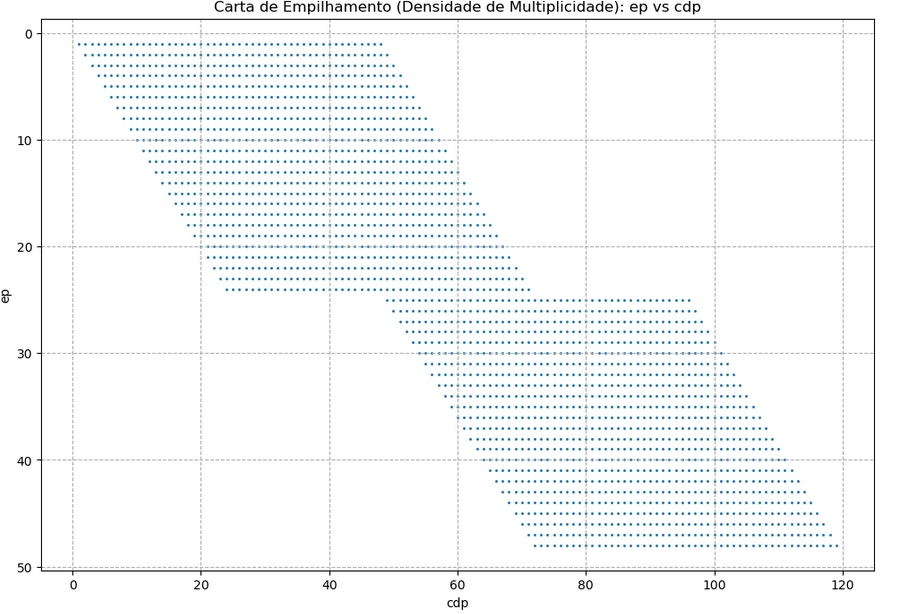
\includegraphics[width=0.75\linewidth]{carta_base_fixa.png}
    \caption{Carta de empilhamento da base fixa.}
    \label{fig:placeholder}
\end{figure}

\subsection{II.4) Questões:}

\subsubsection{1) Qual a janela de afastamentos do primeiro CMP com a multiplicidade de 2400\%?}

Uma janela de afastamento é o conjunto de valores de offset $\rho$ que amostram um determinado CDP, com $\rho = X_G  - X_S$. Sendo assim, por todos pontos amostrarem um único CMP, a posição do CMP deve ser constante. 

O afastamento mínimo $\rho_{min}$ será dado pelo tiro mais longe e pelo geofone mais próximo. A posição do tiro máximo é $X_{S_{24}} = 0 + 23 \cdot 1 = 23m$. Isolando $X_g$ na equação de obtenção da coordenada do CMP, sabendo que $X_{CMP_{24}} = 26.5$, obtemos:

$$X_G = 2\cdot X_{CMP} - X_S = 2 \cdot 26.5 - 23 = 30m$$

Agora, calculando $\rho_{min}$:

$$ \rho_{min} = X_G - X_S = 30 - 23 = 7m$$. 



O afastamento máximo $\rho_{max}$ será dado pelo tiro mais próximo e o geofone mais longe. A posição do primeiro tiro é $X_S = 0m$. Calculando $X_G$, obtemos um valor de $X_G = 2 \cdot 26.5 - 0 = 53m$. Portanto, a janela de afastamentos é $[7, 53]m$.


\subsubsection{2) a) Após a realização de 24 pontos de tiro, qual a janela de afastamentos do último CMP com a multiplicidade de 2400\%?}


O último geofone da base 1 está localizado em $X_G = 77m$. Calculando seu $X_{CDP}$, chegamos em $38.5m$, correspondente ao índice $i = 48$. De forma análoga ao item anterior, calcula-se $X_G$ obtendo o valor de $54m$. Portanto, também de forma análoga ao item anterior, obtemos $\rho_{min} = 54 - 23 = 31m$.

O afastamento máximo se dará quando a fonte e o geofone estiverem na maior distância possível. $X_G = 2 \cdot 38.5 - 0 = 77m$.

Portanto, a janela será de $[31,77]m$.




\subsubsection{b) E qual a janela de afastamentos do CMP seguinte, após a realização de um novo ponto de tiro?}


Com o tiro 25 na posição $24m$ (o último tiro da base 1 está em $23m$), o início da base em $54m$ e o fim da base em $77m$, o afastamento mínimo se dará pela fonte mais a direita e o recepto mais próximo. Calculando: $\rho_{min} = 54 - 24 = 30m$.

O afastaento máximo se dará pelo tiro mais a esquerda e a fonte mais distante: $\rho_{max} = 77 - 1 = 76m$. Logo, a janela é $[30, 76]m$.


\subsubsection{3) Qual o comprimento da linha sísmica em superfície?}

O comprimento é de $101m$. 


\subsubsection{4) Quais as coordenadas do início e final da amostragem em subsuperfície com máxima multiplicidade?}


O início é em $X_{CMP_{24}} = 26.5m$. O final se dará por 

$$ \frac{24 + 101}{2} = 62.5m$$




\subsubsection{5) Descreva duas possibilidades para mudar os parâmetros da geometria de aquisição acima de modo que a multiplicidade máxima fosse 1200\%.}


Pode-se reduzir o número de geofones ou aumentar o intervalo entre tiros, assim manipulando a equação de $M$ para obter o valor desejado. 


\end{document}